% % % % % % % % % % % % % % %
\documentclass[11pt]{article}
\usepackage[a4paper, portrait, margin=1in]{geometry}
\usepackage{adjustbox}
\usepackage{multirow}
\usepackage{booktabs}
\usepackage{adjustbox}
\usepackage{hyperref}
\usepackage{listings}
\usepackage{fancyvrb}
\usepackage{moreverb}
\usepackage{xcolor}
\usepackage{listings}
\usepackage{tcolorbox}
\usepackage{color, colortbl}
\usepackage{float}
\usepackage{cleveref}
\usepackage[toc,page]{appendix}
% % % % % % % % % % % % % % %

\definecolor{swotW}{RGB}{247,193,139}
\definecolor{swotO}{RGB}{173,208,187}
\definecolor{swotT}{RGB}{192,165,184}
%\definecolor{myblue}{rgb}{0.54, 0.81, 0.94}
\definecolor{myblue}{rgb}{0.63, 0.79, 0.95}
\definecolor{mypink}{rgb}{1.0, 0.99, 1.0}



\begin{document}

\title{Advanced Systems Lab (Fall'15) -- Second
Milestone}

\author{Name: \emph{Rabeeh Karimi Mahabadi}\\Legi number: \emph{13-923-941}}

\date{
\vspace{4cm}
\textbf{Grading} \\
\begin{tabular}{|c|c|}
\hline  \textbf{Section} & \textbf{Points} \\ 
\hline  1 &  \\ 
\hline  2 &  \\ 
\hline  3.1 &  \\ 
\hline  3.2 &  \\ 
\hline  4 &  \\ 
\hline  5 &  \\ 
\hline \hline Total & \\
\hline 
\end{tabular} 
}

\maketitle
\newpage


\section{System as One Unit}\label{sec:system-one-unit}

In this section, M/M/1 queuing model of the system based on the stability trace
obtained in first milestone is built. M/M/1 queue can be used to model single 
processor systems or individual devices in a computer system with assumption that 
interarrival times and service times are exponentially distributed, and there 
is only one server. In this experiment, 40 clients, 2 middleware nodes, and one database
instance were used, and a load of mixture of \emph{Pop} and \emph{Write} were used. Clients 
send their requests with fixed rate of 100 \emph{requests/second}. The logs of this 
experiment can be found in \emph{logs/stability\-2}. More details on this experiment can 
be found in \cite[section~3.1]{ms1}.
In order to build the model, mean arrival rate $\lambda$ and mean
service rate $\mu$ should be calculated. To measure service rate, extensive 
log files of stability experiment are collected, and time spent in different 
parts of the system such as front-end, back-end, ... are measured. For more details 
please refer to \cref{sec:stability}. For analyzing log files, a Python script
\emph{analyze/compute\_server\_statistics.py} is written.

To compute mean service time, sum of the the time spent in frontend and backend thread are considered.
Note that time spent waiting in a queue does not count as service time. Table \ref{tbl:mm1-service-time}
shows the average time spent in front-end, and back-end thread, computation of service rate, and average
measured queuing time.

\begin{table}[!ht]
  \begin{tabular}{*3l}    \toprule
    \emph{Name}   & \emph{Value} \\
    \hline
      Backend Thread     & 4.9013 ms \\
      Frontend Thread    & 0.0013 ms \\
      Total time         & 4.9026 ms \\
    \hline
      Service Rate       & 1.0/(4.9026 ms) = 203.9725 requests/second \\
      Mean waiting time  & 4.2076 ms \\ 
    \hline
  \end{tabular}
  \centering
  \caption{Computing service rate of system based on the trace of stability experiment}
  \label{tbl:mm1-service-time}
\end{table}

Computed service rate of $\mu_t=203.9725$ requests per second is much 
smaller than average throughput of system which is $3988.1233$ requests per second. 
This may seem odd at first glance, but can be explained by the structure of the system. In stability experiment, 2 middleware nodes, each of them 
with 10 backend threads(each one has its own database connection) are used. 
Hence, $\mu_t=203.9725$ is the service rate of one backend thread, and total service rate 
is $\mu = 20 \times 203.9725 = 4079.4508 \; requests/second$. which is very 
close to the measured throughput in stability experiment. Therefore, I modeled the system
using 20 M/M/1 queues. For computing $\lambda$, average throughput of stability expeirment is used: $\lambda$=3988.1233.
Table \ref{tbl:mm1-computation} shows computation of different parameters of model.

\begin{table}[ht]
\centering
\begin{tabular}{|c|c|c|c|c|}
\hline
\rowcolor{myblue}
$\rho=\frac{\lambda}{\mu}$&${\rho}_0=1-\rho$& $E[n]=\frac{\rho}{(1-\rho)}$& $Var[n]=\frac{\rho}{(1-\rho)^2}$ & $E(r)=\frac{1}{\mu(1-\rho)}$ \\
\hline
\rowcolor{mypink}
0.9776     &  0.0224  & 43.6628 & 1948.3418 & 10.9496 (ms) \\
\hline
\rowcolor{myblue}
$Var[r]=\frac{1}{\mu^2(1-\rho)^2}$ & $E(w)=\frac{\rho}{\mu(1-\rho)}$ &
$Var[w]=\frac{(2-\rho)(\rho)}{\mu^2(1-\rho)^2}$ &$E[n_q]=\frac{\rho^2}{(1-\rho)}$&
$Var[n_q]=\frac{\rho^2(1+\rho-\rho^2)}{(1-\rho)^2}$\\
\hline
\rowcolor{mypink}
0.00012 & 10.7045 (ms)& 0.00012 &42.6652 & 1946.4085\\
\hline
\end{tabular}
\centering
\caption{Computation of parameters for 20 parallel M/M/1 model of system}
\label{tbl:mm1-computation}
\end{table} Where $\rho$ is traffic intensity, ${\rho}_0$ is probablity of zero job in system, $E[n]$ is 
mean number of jobs, $Var[n]$ is variance of number of jobs in the system,
$E(r)$ is mean response time of the system, $Var[r]$ is variance of response 
time, $E(w)$ is mean waiting time, $E[n_q]$ shows mean number of jobs in the queue, and
$Var[n_q]$ denotes variance of number of jobs in the system.

From table \ref{tbl:mm1-computation}, it can be observed that traffic intensity of system is smaller than 1, therefore,
it satisfies the stability condition. The value of the traffic internsity shows that system was overloaded 
in this experiment. Probablity of all terminals being idle is ${\rho}_0=$0.0224 which is very low, so there is 
a very low probablity that system will be idle. Mean number of jobs in queue in model is $E[n]=$43.6628, 
in the real system 4000 requests per second are applied to the system and mean service time is 
$4.9026 \times 20 = 98.0519(ms)$, therefore on average $\frac{4000}{98.0519}=40.7947$ jobs are 
in system, which is very close to the estimated number in the model. Mean response time of model 
is $E(r)=$10.9496(ms), but, measured mean response time in system is 9.6963 (ms), which
is a bit smaller than the model. This can be explained by the fact that
a system with a single queue performs better than the system with m queues because jobs waiting in the 
queue do not benefit if a thread in another queue is free. Therefore, as the system is modeled with 20 
parallel M/M/1 queues, more response times are expected than the real system. Variance of response 
time in model is very low $Var[r]=$0.00012, however, the measured variance of response-time in 
real system is 3.2546. This can be explained by the fact that, traffic intensity in this experiment
is very close to one, so system is very overloaded, and has reached its maximum capacity. Therefore,
system is expected to struggle handling requests, and more variance in response time is expected.
Another interesting value obtained from \emph{M/M/1} Queue model is mean waiting time $E(w)=$10.7045(ms), 
however, in real system mean waiting time in queue is measured as 4.2076 (ms) \ref{tbl:mm1-service-time}.
Larger mean waiting times in model can be explained in the same manner as larger response times in the model.
Variance of waiting time in model is 0.00012, however, measured variance of waiting time 
in real system is 0.1013 which is higher than the model. The reason for higher variance in waiting time
can be explained similar to the higher variance in response time. Mean number of jobs in queue
in the model is $E(n_q)=$42.6652, for computing mean number of jobs in queue for real system, 
we know that 4000 \emph{request/second} is applied on the system, and mean waiting time in queue 
is 4.2076 (ms) \ref{tbl:mm1-service-time}. Therefore, mean number of jobs in queue will be
16.8304, which is smaller than the estimated value of the model. The reason for having less 
jobs in queue in the real system can be explained again with the difference between 
the real system structure and modelling the system with m parallel M/M/1 queues.


\section{Analysis of System Based on Scalability Data}\label{sec:analysis-scalability}

In this section, M/M/1 queue model of system based on scalability data is presented.
As also done in the previous section, I used m parallel M/M/1 queues to model the system, 
where \emph{m} is number of available worker threads. In scalability experiment, 
throughput and response time of system are measured for varying number of clients(32-960) 
and varying number of middleware nodes(1-2). Number of database connections is fixed at 16.
For more details, please refer to \cref{sec:scalability}.
The measured throughputs and response times are shown in figures \ref{fig:scalability-res}, \ref{fig:scalability-thr}. 
The results show that system has maximum throughput for around 160 clients. Also, as it is 
shown in the figures, there is not that much difference between the throughput and response times of one middleware 
and two middleware nodes experiment. Because of using non-blocking I/O as shown in \cite[section~1.2.4]{ms1}, 
one middleware instance separately can easily handle up to 18500 requests per second.

\begin{figure}[H]
  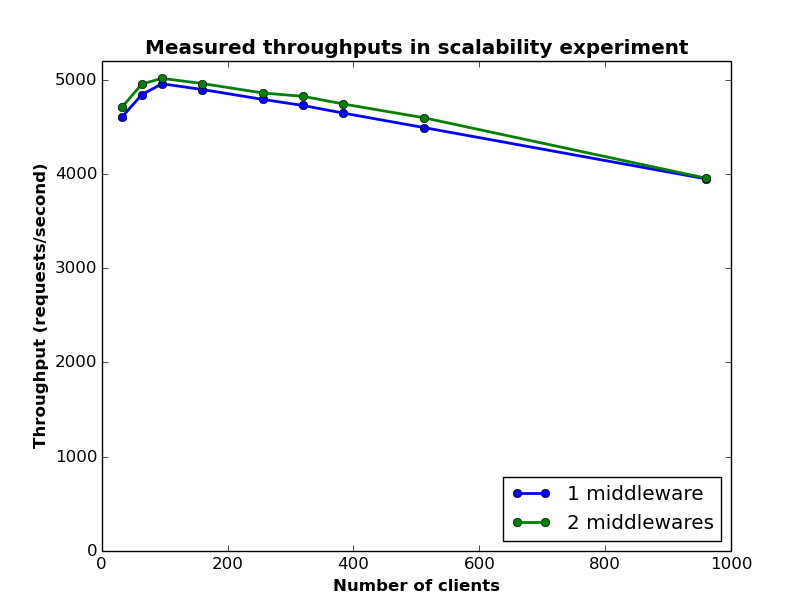
\includegraphics[width=0.6\textwidth,page=1]{figures/mm1/scalability-new/throughput}
  \centering
  \caption{Measured throughput of system in scalability experiment for varying number of clients(32-960), and varying
  number of middleware nodes(1-2). Number of database connections is fixed at 16. System reaches its maximum throughput
  for 160 clients. For more clients, the throughput of system start dropping. Throughput of system for 2 middleware 
  nodes is only slightly higher than one middleware node. As one middleware can easily handle up to 18500 requests 
  per second.}
  \label{fig:scalability-thr}
\end{figure}

\begin{figure}[H]
  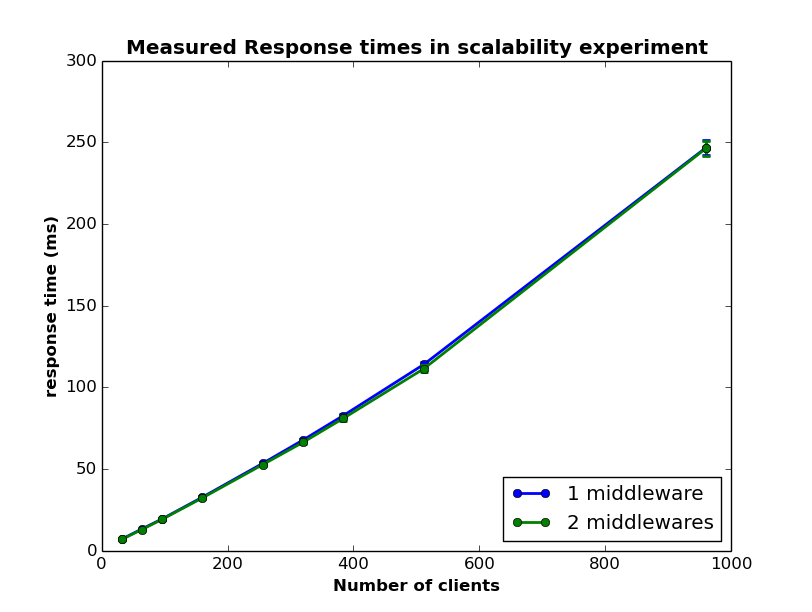
\includegraphics[width=0.6\textwidth,page=1]{figures/mm1/scalability-new/response-times}
  \centering
  \caption{Measured response times of system in scalability experiment for varying number of clients(32-960), and varying 
  number of middleware nodes(1-2). Number of database connections is fixed at 16. By increasing the number 
  of clients, the response time increases, response time increases substantially for more than 160 clients. Obtained 
  response times for one middleare is only slightly higher than 2 middleware nodes.}
  \label{fig:scalability-res}
\end{figure}


In the remainder of this section, models for two different configurations used in 
scalability experiments are presented, then their results with real system are compared.
First, service rate, $\mu$, for different configurations should be calculated.
I logged the times spent in different parts of system for both configuration with 160 clients. The raw data can be found in 
\emph{logs/scalability-new} folder. Table \ref{tbl:scalability1-sr}, \ref{tbl:scalability2-sr}
show backend and front-end thread time, as well as service rate computations for these two configurations. 

\begin{table}[!ht]
  \begin{tabular}{*3l}    \toprule
    \emph{Name}   & \emph{Value} \\
    \hline
      Backend Thread     & 3.2261 ms \\
      Frontend Thread    & 0.0006 ms \\
      Total time         & 3.2267 ms \\
    \hline
      Service Rate       & 1.0/(3.2267 ms) = 309.9152 requests/second \\
    \hline
  \end{tabular}
  \centering
  \caption{Calculation of service rate for 1 middleware node configuration}
  \label{tbl:scalability1-sr}
\end{table}

\begin{table}[!ht]
  \begin{tabular}{*3l}    \toprule
    \emph{Name}   & \emph{Value} \\
    \hline
      Backend Thread     & 3.2254 ms \\
      Frontend Thread    & 0.0007 ms \\
      Total time         & 3.2261 ms \\
    \hline
      Service Rate       & 1.0/(3.2261 ms) = 309.9692 requests/second \\
    \hline
  \end{tabular}
  \centering
  \caption{Calculation of service rate for 2 middleware nodes configuration}
  \label{tbl:scalability2-sr}
\end{table}

As only three values in my scalability experiment were before saturation of system, to better compare the 
behavour of system with the model, I measured more values for this experiment. 
For more details, please refer to  \cref{sec:scalability-additional}.
Tables \ref{tbl:mm1-sclability-1}, and \ref{tbl:mm1-sclability-2} show the calculation of M/M/1 model for scalability 
experiment. For doing the calculation, I wrote a Python script \emph{analyze/mm1.py}.

\begin{table}[!ht]
  \begin{tabular}{*5l}    \toprule
  \emph{N} & \emph{$\lambda(X[Reqs/s])$} &  \emph{$\rho$}  &\emph{$R_{measured}$[ms]} & \emph{$R_{calculated}$[ms]}\\\midrule
8  & 3376.377 & 0.6809 &  2.50526 & 0.632005 \\
16 & 4564.96   & 0.9206 &  3.79030 & 2.540113 \\
32 & 4600.187  & 0.9277 &  7.10450 & 2.789744 \\
48 & 4939.493  & 0.9961 &  9.83219 & 52.21968 \\
96 & 4955.583  & 0.9994 & 19.4420 & 326.8116 \\
    \hline
  \end{tabular}
  \centering
  \caption{Computation for M/M/1 queue model for scalability data with 1 middleware}
  \label{tbl:mm1-sclability-1}
\end{table}

\begin{table}[!ht]
  \begin{tabular}{*5l}    \toprule
   \emph{N} & \emph{$\lambda(X[Reqs/s])$} &  \emph{$\rho$}  & \emph{$R_{measured}$[ms]} & \emph{$R_{calculated}$[ms]}\\\midrule
8   & 3510.56   & 0.7078 &  2.54368& 0.69016 \\
16  & 4382.5466 & 0.8836 &  3.87204& 1.73322 \\
32  & 4704.0233 & 0.9485 &  6.93818& 3.91414 \\
64  & 4952.8333 & 0.9986 &  13.0050& 149.842 \\
160 & 4958.0566 & 0.9997 &  32.3161& 689.478 \\
\hline
  \end{tabular}
  \centering
  \caption{Computation for M/M/1 queue model for scalability data with 2 middlewares}
  \label{tbl:mm1-sclability-2}
\end{table}

Tables \ref{tbl:mm1-sclability-1}, and \ref{tbl:mm1-sclability-2} show that as we add more clients, $\rho$ in 
model get closer to 1. Figures \ref{fig:mm1-scalability-1}, \ref{fig:mm1-scalability-2} show response time of M/M/1 queue
model, as well as real system for scalability experiment. Response times of model have the same trend as measurement values,
but estimated response times are at first smaller than the real system, this can be due to the fact that overhead
of message serialization, coding and decoding, as well as overhead of network is not considered in model. After that, 
response times in model increase very fast with adding more number of clients, however response times in real system,
does not increase this fast. The reasoning is that as we add more clients, and traffic intensity $\rho$ get closer to 1,  
dominator of response time in model get closer to 0, and response times get very large. Response times are calculated with
$E(r)=\frac{1}{\mu(1-\rho)}$ formula in M/M/1 model. However, in real system, when we add more clients, 
the throughput of system does not increase after reaching its maximum throughput, and throughput starts dropping 
when number of requests are more than system capacity as there are not enough connections to handle all
requests. 
Moreover, the other reason for this behavior is that system is modeled as 
\emph{m} separate M/M/1 queues, but real system uses only one queue per middleware instance.
A system with a single queue performs better than system with m queues because 
jobs waiting in queues in \emph{m} parallel M/M/1 queues do not benefit if a thread in another queue is free.


\begin{figure}[H]
  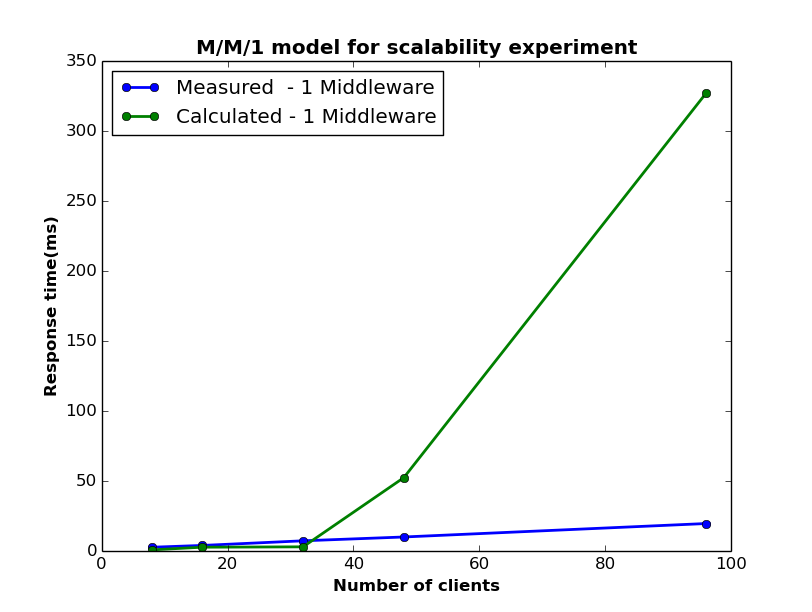
\includegraphics[width=0.6\textwidth,page=1]{figures/mm1/scalability-new/mm1-scalability-1}
  \centering
  \caption{Response times of M/M/1 model and real system for scalability experiment with 1 middleware}
  \label{fig:mm1-scalability-1}
\end{figure}

\begin{figure}[H]
  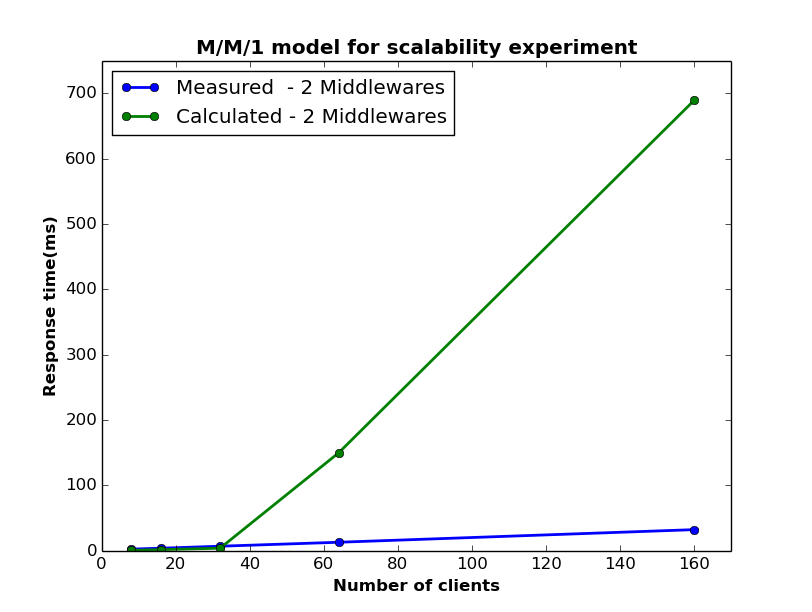
\includegraphics[width=0.6\textwidth,page=1]{figures/mm1/scalability-new/mm1-scalability-2}
  \centering
  \caption{Response times of M/M/1 model and real system for scalability experiment with 2 middlewares}
  \label{fig:mm1-scalability-2}
\end{figure}

\section{Modeling Components as Independent Units}\label{sec:independent-units}

In this section, M/M/m queue models of database and middleware are presented. Then, the results of model 
with real system is compared. M/M/m queue model can be used to model multiprocessor systems or 
devices that have several identical servers and all jobs waiting for these servers are kept in one queue.
M/M/m model is specified with arrival rate $\lambda$ which is jobs per unit time, service rate 
$\mu$ in jobs per unit time, and number of servers \emph{m}. All calculations are done with a Python script 
\emph{analyze/mmm.py} . 

\subsection{Middleware}

In order to model middleware with M/M/m queue model, value of parameters $\lambda$, 
\emph{m}, and $\mu$ should be obtained. The number of parallel servers \emph{m} is set to 30 because I used 30 
front-end threads in my middleware experiment in milestone 1 \cite[section~1.2.4]{ms1}. 
Moreover, middleware instances for \emph{Echo} requests used in this experiment, just read the message and send it back
to clients, so most of the time is spent doing network I/O. Therefore,
having only 2 vCPUs in the \emph{t2.medium} instance of EC2 does not limit performance of middlewares,
and we can choose \emph{m} as 30. To compute the service rate, I used the maximum obtained throughput 
in middleware experiment \cite[section~1.2.4]{ms1}, which was $18441.92$ so considering 
that we have 30 servers, the service rate of $\mu$ is $614.7307$. In order to get a better comparison 
between system and model, I added one more measurements. For more details, please refer to \cref{sec:middleware}.
Table \ref{tbl:mmm-middleware} shows calculation for computing M/M/30 model of 
middleware. 

\begin{table}[!ht]
  \begin{tabular}{*5l}    \toprule
  \emph{N} & \emph{$\lambda(X[Reqs/s])$} &  \emph{$\rho=\lambda/(m \mu)$}  & \emph{$R_{measured}$[ms]} & \emph{$R_{calculated}$[ms]}\\\midrule
4  & 13526.48   & 0.7335  & 0.2951 & 1.7760 \\
8  & 15337.9372 & 0.8317  & 0.5170 & 1.8947 \\
16 & 17848.9833 & 0.9679  & 0.8838 & 3.2598 \\
64 & 18356.9042 & 0.9954  & 3.4882 & 13.3719 \\
\hline
  \end{tabular}
  \centering
  \caption{computation of M/M/30 model for middleware experiment}
  \label{tbl:mmm-middleware}
\end{table}


Figure \ref{fig:mmm-middleware} shows response time of model and real system measured in middleware experiment. 
While calculated response times are higher than measured response times, the general 
trend is very similar to the behaviour of system. Higher response times in model can be because of the fact that 
in M/M/m model, assumption is that all of the jobs waiting for servers are kept 
in one queue. However, middleware in real system, uses nonblocking network I/O in 
combination with multi-threading. Therefore, M/M/30 model is only a rough approximation
as in this model, most of the network I/O is done in one thread.
So it make sense for me, that because system uses nonblocking I/O and handle requests 
asynchronously, it has less response time than calculated respose times in model. 

\begin{figure}[H]
  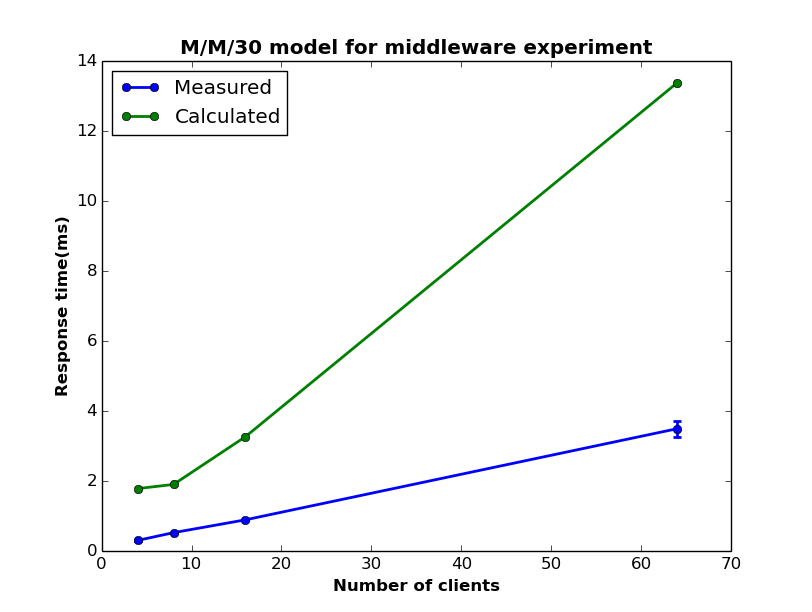
\includegraphics[width=0.6\textwidth,page=1]{figures/mmm/mmm-middleware}
  \centering
  \caption{M/M/30 model for Middleware based on the middleware experiment \cite[section~1.2.4]{ms1}}
  \label{fig:mmm-middleware}
\end{figure}


\subsection{Database}
\label{sec:report-database}

To model database with M/M/m model, value of parameters $\lambda$, $\mu$, and $m$ should be obtained. 
For my experiments, I used \emph{m3.large} instance with \emph{2} \emph{vCPUs} to run 
database. For more details on this experiment, please refer to \cref{sec:database}.
I set \emph{m} in the queuing model to 2. The reasoning is that although 2 vCPUs do not 
directly map to 2 CPU cores, but they behave similar to 2 cores of an Intel Xeon E5-2670 
\footnote{\url{http://aws.amazon.com/ec2/instance-types/}}. Hence, the system should be able to 
handle 2 requests cocurrently.

For computing service rate of the database, I used the maximum measured throughput in database combination load 
experiment in \cref{sec:database}. Maximum throughput of this experiment was 5023.74074 \emph{requests/second}. I used this number as total
service rate. So, each individual server has service rate of $\mu$=2511.8704 requests per second.

Table \ref{tbl:mmm-database} shows calculated response times of model, traffic intensity, as well as 
measured response times of combination load database experiment. 
\begin{table}[!ht]
  \begin{tabular}{*5l}    \toprule
  \emph{N} & \emph{$\lambda(X[Reqs/s])$} &  \emph{$\rho=\lambda/(m \mu)$}  & \emph{$R_{measured}$[ms]} & \emph{$R_{calculated}$[ms]}\\\midrule
4   & 2100.6778 & 0.4182  & 1.8684 & 0.5412 \\
8   & 3705.9296 & 0.7377  & 2.1156 & 0.9579 \\ 
16  & 4702.0222 & 0.9360  & 3.4153 & 3.3074 \\
24  & 4745.9111 & 0.9447  & 5.2163 & 3.7984 \\
40  & 4989.6422 & 0.9932  & 8.4503 & 29.5258 \\
\hline
  \end{tabular}
  \centering
  \caption{Computing M/M/2 model for database combination load experiment}
  \label{tbl:mmm-database}
\end{table}

As shown in table \ref{tbl:mmm-database}, all traffic intensity values $\rho$ are less than 1, meaning that 
system is stable. Figure \ref{fig:mmm-database} shows the response times of real system and the 
computed values from M/M/2 model.
\begin{figure}[H]
  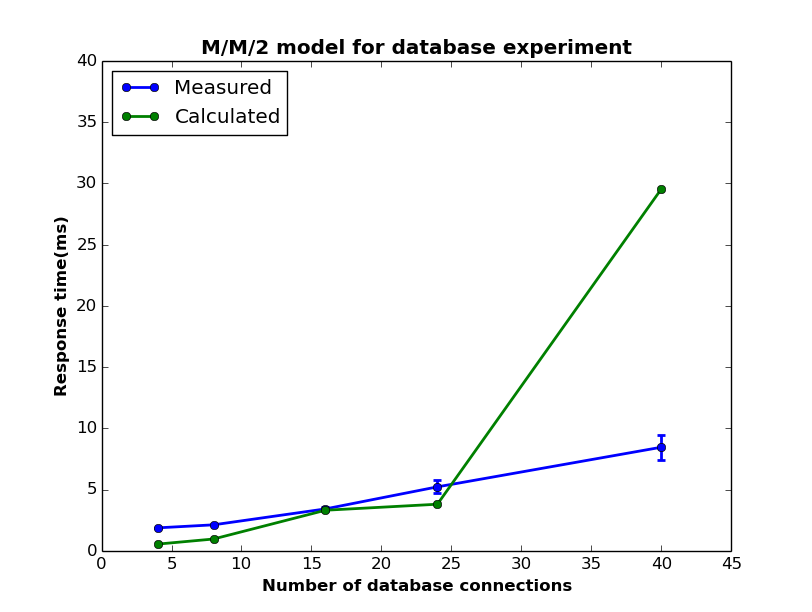
\includegraphics[width=0.6\textwidth,page=1]{figures/mmm/mmm-database}
  \centering
  \caption{Response times for M/M/2 model and real system for database experiment. In this experiment a 
   combination of \emph{read} (50 $\%$), \emph{write} (25 $\%$), and \emph{send} (25 $\%$) are used, 
   and response-times for  different number of database connections are measured.}
  \label{fig:mmm-database}
\end{figure}

As shown in figure \ref{fig:mmm-database}, measured values clearly follow the trend of the built model.
However, there are some differences, at first model predicts smaller values for response times 
than real response times, and this is because of the fact that model does not consider overhead 
of the network, serialization, coding and decoding of messages.
Another point we can see from this graph is that, by adding more database connections in the model, 
and as traffic intensity get closer to 1,  response times increase a lot. However, in real 
system, increase in reponse-times is not that drastic. The reasoning is that, 
adding a lot of database connections to system, results in drop of throughput in reality.
Each connection is handled by a separate process in Postgresql, and more 
connections lead to more locking and process switching overhead. Therefore, having more database 
connections does not translate diretly to having more throughput, and results in a drop 
in performance, so traffic intensity close to 1 in reality does not occur. However, 
in model, as lambda get closer to service rate, and $\rho$ get closer to 1, 
based on formula of response time $E(r)=\frac{1}{\mu}(1+\frac{\rho}{m(1-\rho)})$, it results in a huge 
increase in response-time values. So, raw number of requests per second is not the only limiting factor, 
and model does not consider number of connections to database which is an important 
limiting factor. 

\section{System as Network of Queues}\label{sec:network-of-queues}

In this section, the whole system is modeled with a network of queues. In my
first attemp, I used the model described in \cite[section~34.2]{book}. 
Most important parts of my system are clients, network I/O, front-end threads in middleware, 
back-end threads, and database which are all modeled using queues. I used the results of 
maximum throughput experiment in first milestone to model my system. In this experiment, 
I used 2 middlewares, each with 30 front-end pool workers, and 16 database connections. 
A workload of combination of \emph{pop}, \emph{peek}, \emph{send}, and \emph{query}, each with 
equal portion is used. Client think time is set to zero. Figure \ref{fig:queue-structure} shows considered structure of queueing network for modelling the whole 
system. I analysed the network, with mean value analysis algorithm described in \cite[section~34.2]{book}, and I wrote 
a Python code for it provided in \emph{analyze/mva.py}.

\begin{figure}[H]
  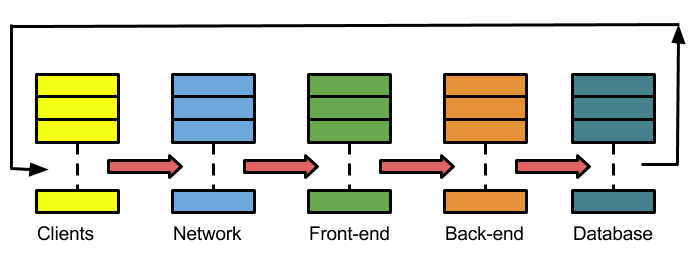
\includegraphics[width=0.6\textwidth,page=1]{figures/structure}
  \centering
    \caption{Queuing network structure of model}
  \label{fig:queue-structure}
\end{figure}

All parameters of model are shown in \cref{tbl:queue-model-1}.

\begin{table}[ht]
\centering
\begin{tabular}{|c|c|}
\hline
\rowcolor{myblue}
Client think time           & 0 (s) \\
\rowcolor{mypink}
Number of network queues    & 60   \\
\rowcolor{myblue}
Network service time        & 0.0766 (s) \\
\rowcolor{mypink}
Network visit rate          & $\frac{1}{60}$\\
\rowcolor{myblue}
Number of front-end threads & 60 \\
\rowcolor{mypink}
Front-end service time      & 0.0008187 (s)\\
\rowcolor{myblue}
Front-end visit rate        & $\frac{1}{60}$ \\ 
\rowcolor{mypink}
Number of worker threads    & 32 \\
\rowcolor{myblue}
worker threads service time & 0.01895 (s)\\
\rowcolor{mypink}
Number of database processes & 2 \\
\rowcolor{myblue}
Database service time        & 0.3981 (s)\\
\hline
\end{tabular}
\centering
\caption{Parameters used in modelling the whole system using network of queues}
\label{tbl:queue-model-1}
\end{table}

As shown in table \ref{tbl:queue-model-1}, for modelling network I/O, I assumed that 
each frontend thread can send and receive data from a single connection. Therefore, 
I modeleted network I/O using 60 queues to simplify the model. As network I/O
has only a negligible impact on overal performance, this choice seems reasonable to me.
For measuring the time spent in different parts of the system, extensive logs of max throughput
experiment are collected. For more information, please refer to \cref{sec:max-throughput}. 
I measured the time spent in different parts of the system using a Python script 
\emph{analyze/compute\_server\_statistics.py} from the logs provided in 
\emph{logs/maxThroughput/max-throughput-with-logs} folder. Network time is measured by adding the time spent for sending a request, and response. Detailed computation 
of network I/O time is shown in table \ref{tbl:network-time}. 

\begin{table}[!ht]
  \begin{tabular}{*3l}    \toprule
    \emph{Name}   & \emph{Value} \\
    \hline
      Front-end waiting time     & 0.0512 ms \\
      Response time              & 0.0071 ms \\
      Response waiting time      & 0.0183 ms \\ 
      \hline
      Total network I/O time     & 0.0766 ms \\
    \hline
  \end{tabular}
  \centering
  \caption{Computation of network I/O time for max throughput experiment}
  \label{tbl:network-time}
\end{table}

As there are two middlware instances, and each of them has 30 front-end threads, I modeled each front-end thread as a single queue, so in total,
I considered 60 queues to model front-end threads in middlewares. For modelling database,
I modeletd each database connection as a single queue, so in total, I considered 32 queues for 
overal database part. Database service time is measured as explained in \cref{sec:report-database}.


 Figures \ref{fig:mva-thr}, and \ref{fig:mva-resp} show the throguhput and response times 
 calculated with MVA algorithm and the real system. The calculated values are very close to the real 
 measured values in the system. However, the throughput calculated using the model is slightly less than the real measured throughputs.
 The reason is that in this model, every component is modelled as m parallel M/M/1 queue. However, in the 
 real system there are less queues. For instance, there is only one front-end queue for each middleware instance,
 but in the model, every front-end thread is modeled with one single queue. Therefore, 60 queues are used 
 to model front-end queue. As explained before, system with a single queue performs better than the system with 
 multiple parallel queues. Because it has less waiting time, but with m-parallel M/M/1 queues, it can happen that 
 while jobs are waiting in one queue, another queue is idle. Because of this reasoning, it is expected 
 that the real system has slightly higher throughputs and less response times.
 
\begin{figure}[H]
  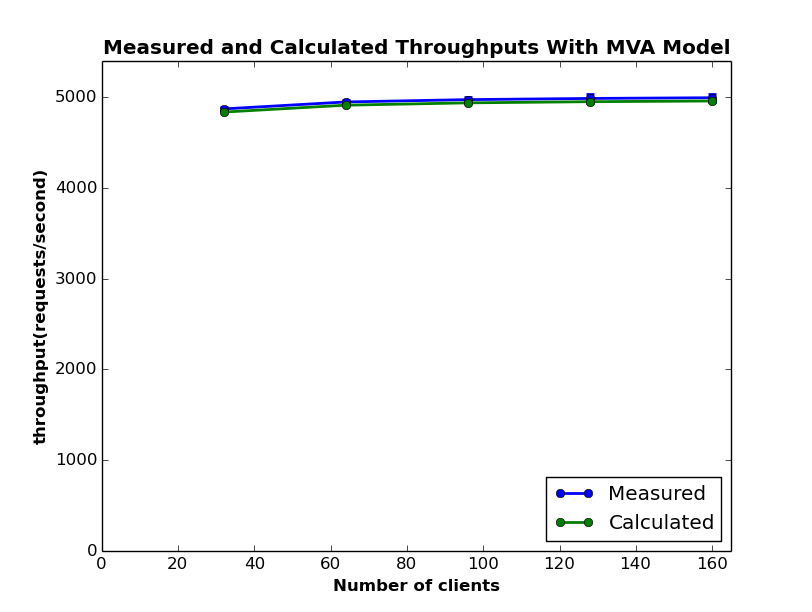
\includegraphics[width=0.6\textwidth,page=1]{figures/mva/throughput}
  \centering
  \caption{Calculated throughputs of the system using MVA algorithm \cite[section~34.2]{book} 
  versus measured throughputs of system.}
  \label{fig:mva-thr}
\end{figure}

\begin{figure}[H]
  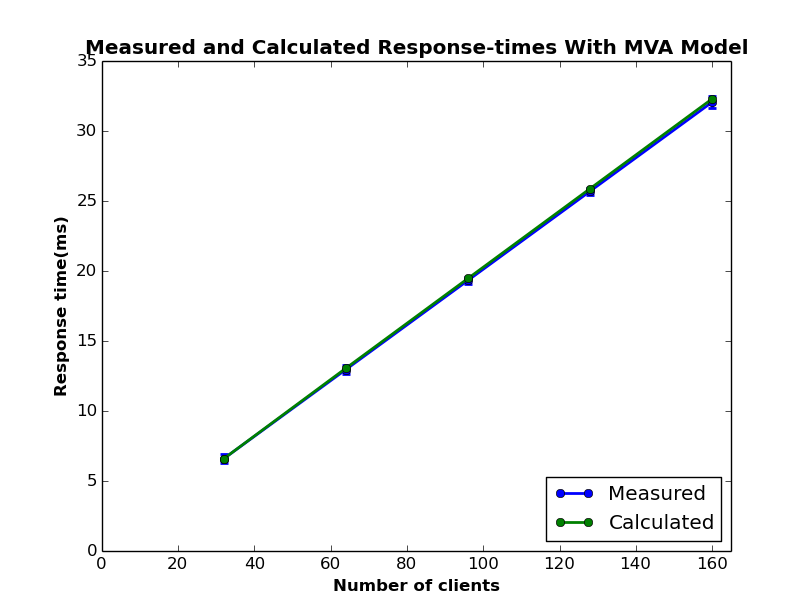
\includegraphics[width=0.6\textwidth,page=1]{figures/mva/response-time}
  \centering
  \caption{Calculated response-times of the system using MVA algorithm \cite[section~34.2]{book} 
  versus measured response-times of system.}
  \label{fig:mva-resp}
\end{figure}

In my second attemp, I tried to model the system using MVA including load dependent centers. I implemented the the algorithm on 
\cite[section~36.1]{book} in a Python code \emph{analyze/mva\_load\_dependent.py}. At first, I modelled network 
I/O using delay centers because we can consider that there is no queuing, and jobs spend the same
amount of time in the device regardless of the number of jobs in it. Therefore, network I/O can be modeled as 
a center with inifinite servers. However, the results accuracy were not good for this model, and I modeled the network 
I/O, as explained in previous model. Front-end, and back-end are also modelled the same as previous model.
However, database is modelled using load-dependent service
center since its service rate is depend upon the load or number of jobs in the device. Service time and number of 
threads for each part of model are the same as previous model, but in this model, number of visits to each device should be 
set to one. For network I/O I measured the round trip time, so it is correct that we set the number 
of visits to 1. Front-end threads are responsible to send the requests to the backend and send back the response to 
clients, however, this does not really count as 2 visits, because in sending back the response to the clients,
the load is very low, and there is not that much indeed happening. Figures \ref{fig:mva-thr-2} and \ref{fig:mva-resp-2} show
the measured throughput and response times in the real system and the ones obtained using the new MVA model.
The obtained values in this model are almost accurate, and the same reasoning as explained in previous model, for having higher 
throughput and less response times in the real system than model is also applied to this model. 
The calculated values in this model are not as accurate as previous model, the reasoning
can be that modelling load dependent servers can be very complex and the algorithm given in \cite[section~36.1]{book}
should be an approximation.

\begin{figure}[H]
  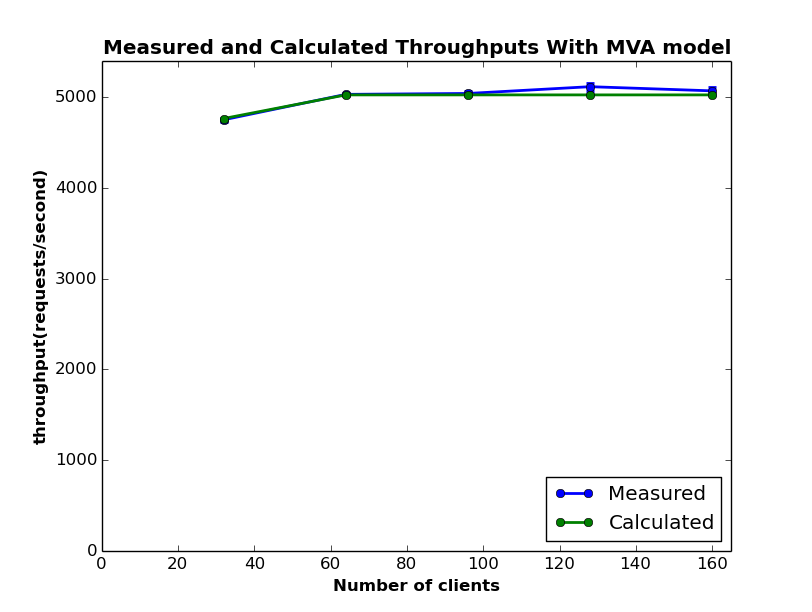
\includegraphics[width=0.6\textwidth,page=1]{figures/mva-load-dependent/throughput}
  \centering
  \caption{Measured and calculated throughputs of system using MVA algorithm with load dependent center for database.}
  \label{fig:mva-thr-2}
\end{figure}

\begin{figure}[H]
  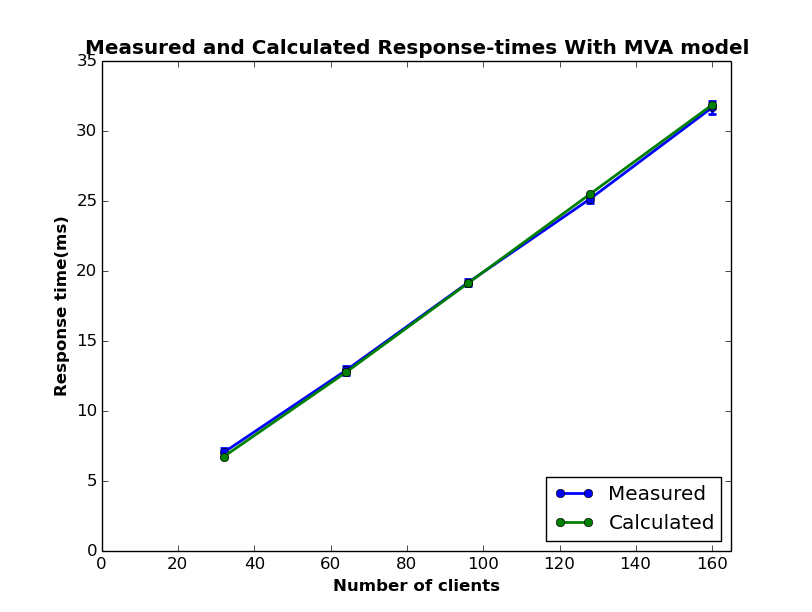
\includegraphics[width=0.6\textwidth,page=1]{figures/mva-load-dependent/response-time}
  \centering
  \caption{Measured and calculated response-times of system using MVA algorithm with load dependent center for  
  database.}
  \label{fig:mva-resp-2}
\end{figure}


\section {Bottleneck Analysis}

As discussed in \cite[section~33.6]{book}, as a consequence of forced flow law, device utilizations are 
proportional to their respective total service demands. The device with highest total
service demand $D_i$, has the highest utilization, and is called bottleneck device. As in MVA algorithm, 
utilizations of devices are already computed, I used utilization values to do the analysis of this section.
Utilizations are computed using a Python script \emph{analyze/mva.py}. Table \ref{tbl:utilization} shows the 
computed utilization values of different components of the system.

\begin{table}[!ht]
  \begin{tabular}{*5l}    \toprule
  \emph{N} & \emph{network I/O} &  \emph{front-end}  & \emph{back-end} & \emph{database}\\\midrule
32	&	0.006220	&0.000066	&0.002883&	0.969243 \\
64	&	0.006318	&0.000067	&0.002928&	0.984499 \\
96	&	0.006351	&0.000068	&0.002944&	0.989639 \\
128	&	0.006368	&0.000068	&0.002951&	0.992219 \\
160	&	0.006378	&0.000068	&0.002956&	0.993770 \\ 
\hline
  \end{tabular}
  \centering
  \caption{Utilization of different parts of system computed using MVA algorithm}
  \label{tbl:utilization}
\end{table}

Figure \ref{fig:utilization} shows the utilization of different components of system.
Clearly, database has the highest utilization, and therefore is the bottleneck device.
For 128 clients, the system has maximum throughput \cite[section~3.3]{ms1} and utilization of database is around 1. In this design, database, has the highest
service time, because, there is only one database instance, and it has to handle queries from all
middleware instances. In addition, using \emph{SELECT FOR UPDATE} for implementing  
\emph{pop} queries limits the performance as once one thread is trying to remove a 
message from database, other threads are blocked. Moreover, inorder to answer queries, database has to read and write 
data from the hard drive which is time-consuming. Using indexes can help in improving the 
efficiency of read, however, still database needs to write all changes to hard drive which
takes time. Therefore, service time of database is very high. Utilization for front-end
threads are even less than the utilization of network I/O. The reasoning is that front-end threads have 
to only parse requests and make the corresponding back-end tasks, and also returning back the 
response to client at the end. Front-end threads are very efficient because they use the non-blocking I/O and message
serialization. 

\begin{figure}[H]
  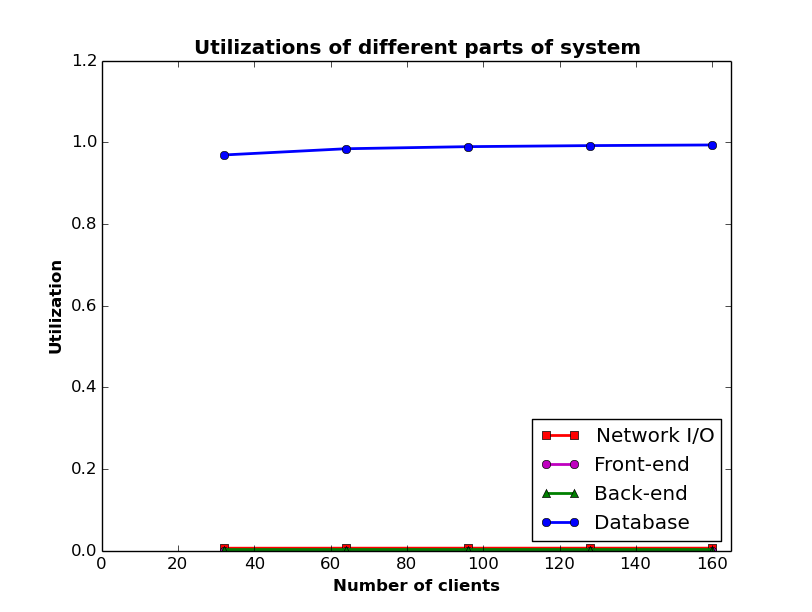
\includegraphics[width=0.6\textwidth,page=1]{figures/utilization/utilizations}
  \centering
  \caption{Utilizations of different components of the system computed using the MVA algorithm.}
  \label{fig:utilization}
\end{figure}

\section{Interactive Law Verification}\label{sec:interactive-law}

In this section, validity of all experiments done is checked using Interactive law. 
Based on interactive reponse time law, we have the following relation:
\begin{equation}
X=\frac{N(\frac{T}{R+Z})}{T}=\frac{N}{R+Z}  
\end{equation} Where \emph{X} represents system throughput, \emph{R} is response-time,
\emph{Z} is think time, \textit{N} is number of users, and \emph{T} shows time period.
Similarly, response time can be calculated using the following relation:
\begin{equation}
R=\frac{N}{X}-Z
\end{equation} I wrote a Python script \emph{analyze/interactive\_law.py} to analyze the data. Response-times 
using the above formula are calculated and compared with the measured response-times. Table \ref{tbl:interactive-db} shows the calculation for 
interactive law verification for database combination load experiment, and 
figure \ref{fig:interactive-db} shows the values on the graph. Since difference between calculated and 
measured response-times is very small, experiment is valid according to the interactive law.


\begin{table}[!ht]
  \begin{tabular}{*7l}    \toprule
    \emph{N}   & \emph{X[Reqs/s]} & \emph{Z[ms]} & \emph{$R_{measured}$[ms]} & \emph{$R_{calculated}$[ms]} &   \emph{Difference[ms]} & \emph{Difference[\%]} \\\midrule

    4 &      2100.6777 &          0 &    1.8683 &    1.9041 &       0.0357  &  1.8783 \\
    8 &      3705.9296 &          0 &    2.1156 &    2.1587 &       0.0387  &  1.9945 \\
    16 &     4702.0222 &          0 &    3.4153 &    3.4027 &       0.0072  &  0.3675 \\
    24 &     4745.9111 &          0 &    5.2162 &    5.0569 &       0.1630  &  3.0535 \\
    36 &     5023.7407 &          0 &    7.5606 &    7.1659 &       0.3553  &  5.2191 \\
    \hline
  \end{tabular}
  \centering
  \caption{Measured and calculated response times for combination load database experiment}
  \label{tbl:interactive-db}
\end{table}

\begin{figure}[H]
  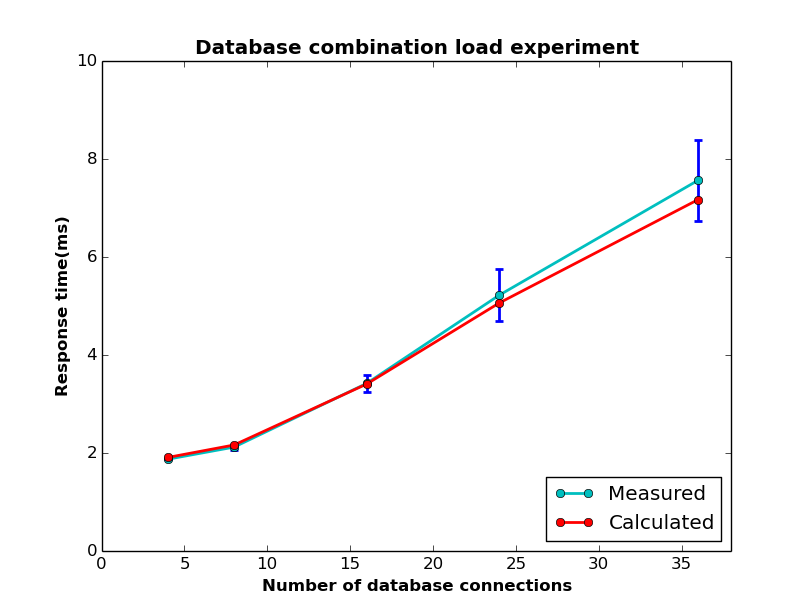
\includegraphics[width=0.6\textwidth,page=1]{figures/interactive_law/db}
  \centering
  \caption{Measured and calculated response times for combination load database experiment}
  \label{fig:interactive-db}
\end{figure}



Table \ref{tbl:interactive-max} shows calculation for 
interactive law verification for maximum throughput experiment, and 
figure \ref{fig:interactive-max} shows the values on a graph. Since difference between calculated and 
measured response-time values is small, experiment is valid according to interactive law.

\begin{table}[!ht]
  \begin{tabular}{*7l}    \toprule
    \emph{N}   & \emph{X[Reqs/s]} & \emph{Z[ms]} & \emph{$R_{measured}$[ms]} & \emph{$R_{calculated}$[ms]} &   \emph{Difference[ms]} & \emph{Difference[\%]} \\\midrule
         32    & 4749.2233      & 0            & 7.0192 & 6.7379  &  0.2812 & 4.0068 \\
         64    & 5029.5733      & 0            & 12.8756& 12.7247 &  0.1509 & 1.1722 \\
         96    & 5039.4566      & 0            & 19.1496 &19.0496 &  0.0999 & 0.5221 \\
        128    & 5114.1966      & 0            & 25.1325 & 25.0283 & 0.1042 & 0.4146 \\
        160    & 5068.2333      & 0            & 31.6622 & 31.5691 & 0.0931 & 0.2940 \\
    \hline
  \end{tabular}
  \centering
  \caption{Measured and calculated response times for maximum throughput experiment}
  \label{tbl:interactive-max}
\end{table}

\begin{figure}[H]
  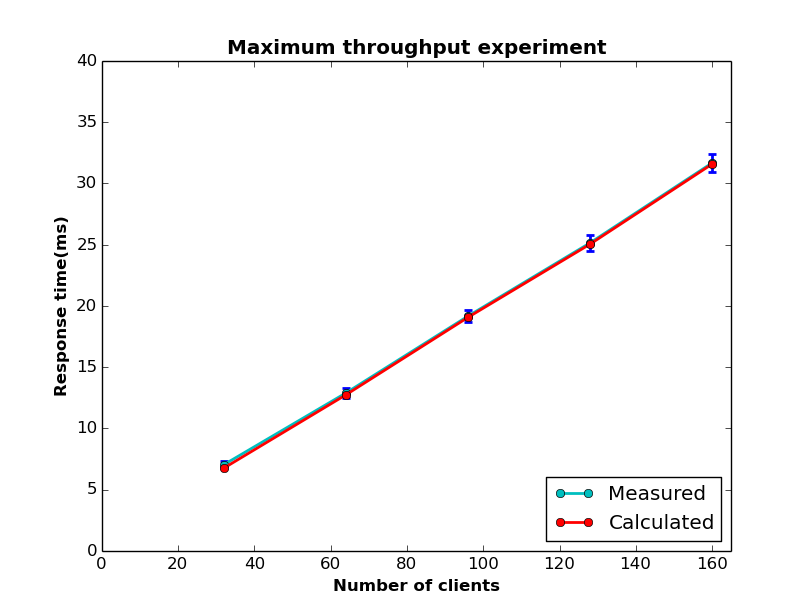
\includegraphics[width=0.6\textwidth,page=1]{figures/interactive_law/maxThroughput}
  \centering
  \caption{Measured and calculated response times for maximum throughput experiment}
  \label{fig:interactive-max}
\end{figure}


Table \ref{tbl:interactive-middleware} shows calculation for 
interactive law verification for middleware experiment \cite[section~1.2.4]{ms1}, and 
figure \ref{fig:interactive-middleware} shows the values on a graph. Difference between calculated and 
measured response-times is small. Therefore, experiment is valid according to interactive law.


\begin{table}[!ht]
  \begin{tabular}{*7l}    \toprule
    \emph{N}   & \emph{X[Reqs/s]} & \emph{Z[ms]} & \emph{$R_{measured}$[ms]} & \emph{$R_{calculated}$[ms]} &   \emph{Difference[ms]} & \emph{Difference[\%]} \\\midrule
   8 & 15337.9372 & 0  & 0.5170 & 0.5216& 0.0045 & 0.8779 \\
   16& 17848.9833 & 0  & 0.8838 & 0.8964& 0.0126&  1.4018 \\
   32& 18441.6542 & 0  & 1.7126 & 1.7352& 0.0226&  1.3043 \\
   64& 18356.9042 & 0  & 3.4882 & 3.4864& 0.0018&  0.0520\\
    \hline
  \end{tabular}
  \centering
  \caption{Measured and calculated response times for middleware experiment}
  \label{tbl:interactive-middleware}
\end{table}


\begin{figure}[H]
  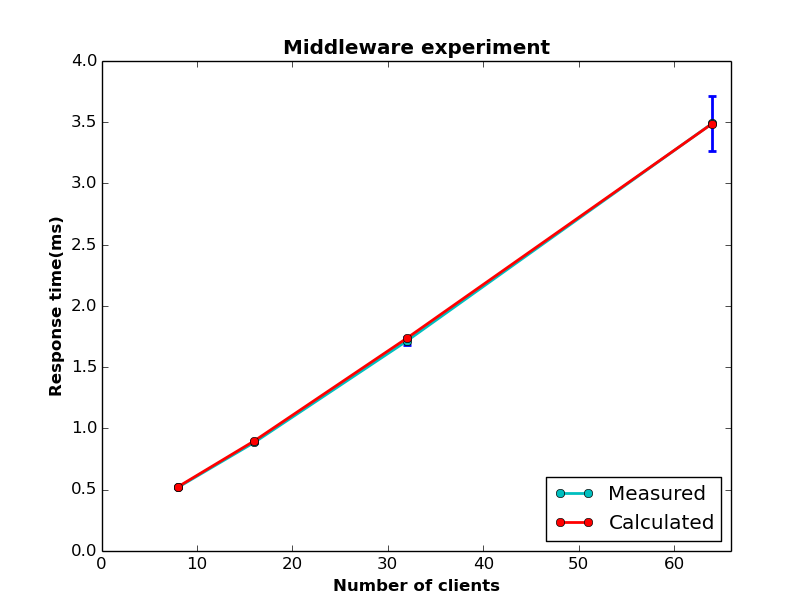
\includegraphics[width=0.6\textwidth,page=1]{figures/interactive_law/middleware}
  \centering
  \caption{Measured and calculated response times for middleware experiment}
  \label{fig:interactive-middleware}
\end{figure}


Table \ref{tbl:interactive-2k} shows the calculation for interactive law Verification 
for 2k factorial experiment  \cite[section~3.2]{ms1}. Difference between calculated and 
measured response-time values is very small. Therefore, experiment is valid according to the interactive law.

\begin{table}[!ht]
  \begin{tabular}{*9l}    \toprule
   \emph{L} &  \emph{M}  & \emph{N} & \emph{X[Reqs/s]} & \emph{Z[ms]} & \emph{$R_{measured}$[ms]} & \emph{$R_{calculated}$[ms]} &   \emph{Difference[ms]} & \emph{Difference[\%]} \\\midrule
       1200 &   1         &  32  & 3903.7033     & 0   & 8.2958 & 8.1973 & 0.0985 & 1.1872 \\
       200  &   1         &  32  & 4003.35       & 0   & 8.0673 & 7.9933 & 0.0740 & 0.9178 \\
       1200 &   2         &  32  & 2518.5166     & 0   & 12.9001& 12.7059& 0.1943& 1.5058 \\
       200  &   2         &  32  & 2544.4983     & 0   & 12.7199& 12.5761& 0.1438& 1.1304\\
       1200 &   1         &  64 &3957.8166 & 0         & 16.2519& 16.1705& 0.0814& 0.5011 \\
       200  &   1         &  64 & 3960.3833&  0        & 16.2053 & 16.1600& 0.0452& 0.2791\\
       1200 &   2         &  64 & 2507.0699& 0         & 25.6467 & 25.5278 & 0.1188& 0.4635 \\
        200 &   2         &  64 & 2547.7316& 0         & 25.2043  & 25.1204 & 0.0839& 0.3329 \\
    \hline
  \end{tabular}
  \centering
  \caption{Measured and calculated response times for $2k$ factorial experiment}
  \label{tbl:interactive-2k}
\end{table} Where \emph{L} represents message length and \emph{M} shows number of middleware nodes.
A number of experiments have been repeated in this experiment, the details are discussed in \cref{sec:2k}.

To verify stability experiment, mean response time for this experiment is measured as  
9.6963 (ms) and mean throughput value is 3988.1233 requests per second. By applying the interactive law: 

\begin{equation}
X=\frac{N}{R+Z} = \frac{40}{9.6963/1000.0} = 4125.2945
\end{equation} 

which has only $3\%$ difference with the measured throughput value. Therefore, this experiment is 
valid based on interactive law. Measured and calculated response times for stability experiment are shown in figure  
\ref{fig:interactive-stability}.

\begin{figure}[H]
  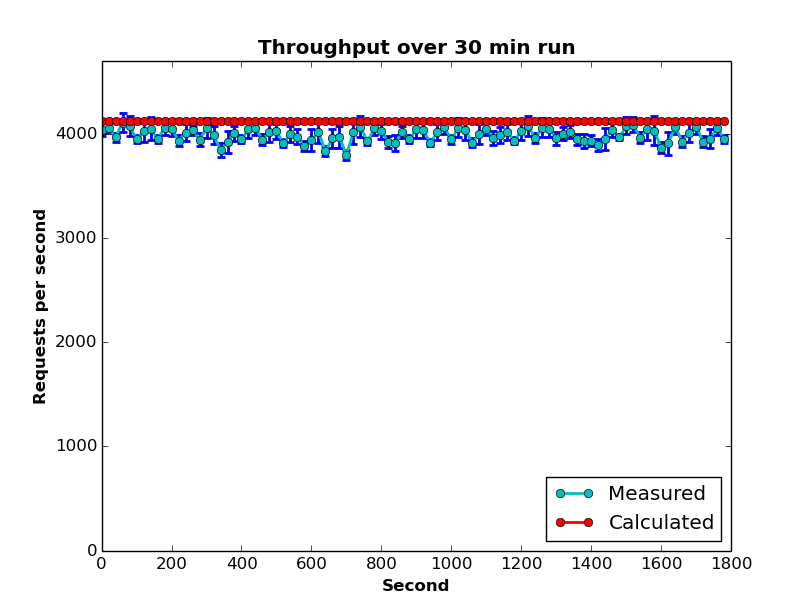
\includegraphics[width=0.6\textwidth,page=1]{figures/interactive_law/stability2}
  \centering
  \caption{Measured and calculated throughput for stability experiment}
  \label{fig:interactive-stability}
\end{figure}



Table \ref{tbl:scalability-1middleware}, and \ref{tbl:scalability-2middlewares} show calculation for 
interactive law Verification for scalability experiment \ref{sec:scalability} for 1 and 2 middleware nodes,
and figure \ref{fig:interactive-scalability} shows the values on a graph. Small difference between measured 
and calculated respose-times shows that experiment is valid according to the interactive law.

\begin{table}[!ht]
  \begin{tabular}{*7l}    \toprule
   \emph{N} & \emph{X[Reqs/s]} & \emph{Z[ms]} & \emph{$R_{measured}$[ms]} & \emph{$R_{calculated}$[ms]} &   \emph{Difference[ms]} & \emph{Difference[\%]} \\\midrule

32 &  4600.1874  & 0 & 7.1045  & 6.9562   & 0.1482 & 2.0870  \\
64 &  4840.8466  & 0 & 13.3158 & 13.2208  & 0.0950 & 0.7135  \\
96 &  4955.5833  & 0 & 19.4420 & 19.3721  & 0.0699 & 0.3594  \\
160&  4894.83    & 0 & 33.5268 & 32.6875  & 0.8393 & 2.5032  \\
256&  4789.8933 & 0 & 53.5082  & 53.4459  & 0.0623 & 0.1165  \\
320 & 4725.1399 & 0 & 67.8064  & 67.7228  & 0.0835 & 0.1232  \\
384 & 4644.3233 & 0 & 82.7717  & 82.6815  & 0.0902 & 0.1089  \\
512 & 4490.7699 & 0 & 114.1421 & 114.0116 & 0.1304 & 0.1143  \\
960 & 3946.1567 & 0 & 246.8159 & 243.2747 & 3.5413 & 1.4348  \\
\hline
  \end{tabular}
  \centering
  \caption{Measured and calculated response times for scalability experiment with 1 middleware}
  \label{tbl:scalability-1middleware}
\end{table} 


\begin{table}[!ht]
  \begin{tabular}{*7l}    \toprule
   \emph{N} & \emph{X[Reqs/s]} & \emph{Z[ms]} & \emph{$R_{measured}$[ms]} & \emph{$R_{calculated}$[ms]} &   \emph{Difference[ms]} & \emph{Difference[\%]} \\\midrule
32 & 4704.0233 & 0 & 6.9382  &  6.8027 & 0.1355     & 1.9528 \\
64 & 4952.8333 & 0 & 13.0050 & 12.9219 & 0.0832     & 0.6393 \\
96 & 5013.1167 & 0 & 19.2039 & 19.1498 & 0.0541     & 0.2817 \\
160& 4958.0567 & 0  & 32.3161 & 32.2707& 0.0454     & 0.1403\\
256 & 4857.8333 & 0 & 52.7461 & 52.6983 & 0.0477    & 0.0904\\
320 & 4822.6533 & 0  & 66.4015 & 66.3535& 0.0481    & 0.0724 \\
384 & 4740.9633 & 0 & 81.0631& 80.9961 & 0.0669     & 0.0825\\
512 & 4594.8899 & 0 & 111.5061 & 111.4281 & 0.0779  & 0.0699\\
960 & 3953.5470  & 0 & 246.4149 & 242.8199 & 3.5949 & 1.4589\\
    \hline
  \end{tabular}
  \centering
  \caption{Measured and calculated response times for scalability experiment with 2 middlewares}
  \label{tbl:scalability-2middlewares}
\end{table} 

\begin{figure}[H]
  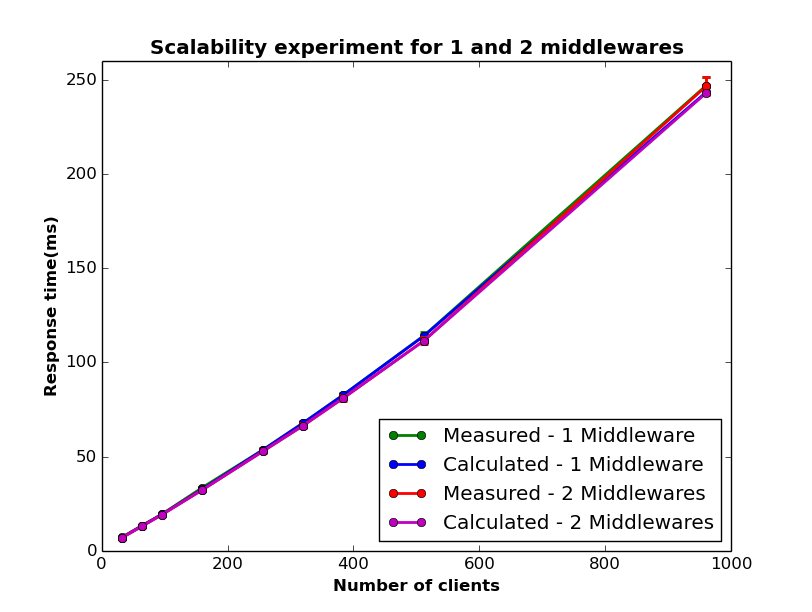
\includegraphics[width=0.6\textwidth,page=1]{figures/interactive_law/scalability}
  \centering
  \caption{Measured and calculated response times for scalability experiment}
  \label{fig:interactive-scalability}
\end{figure}


\begin{appendices}

\section{Appendix: Repeated Experiments}

While most of the data used in this report are obtained in milestone 1, more experiments 
and measurements are performed to collect the necessary data to build the models.

\subsection{Stability Experiment}
\label{sec:stability}

In order to compute service rate of middlewares for stability experiment, the times 
spent in different parts of system are measured. As these values were not needed in  
first milestone, I ran stability experiment with same setting as first milestone
for 5 minutes and logged times spent in different parts of 
system: backend-time, backend-waiting time, front-end time, frontend-waiting 
time, response-time, response-waiting time. These logs can be found in 
\emph{logs/stability-2-with-server-logs} folder. 

\subsection{Scalability Experiment}
\label{sec:scalability}

As my scalability experiment design in first milestone was not sufficient, I ran this experiment again
with a new experimental design. Throughput and response times of system are measured for 
varying number of clients(32-960) and middleware nodes(1-2). The logs can be found in \emph{logs/scalability-new}.
The number of database connections is fixed at 16 because in database 
experiment \cite[section~1]{ms1}, it was shown that using 16 database connections results in maximum performance.
As in first milestone, I used \emph{m3.large} instance for database, \emph{t2.medium} for clients, and two more
\emph{t2.medium} machines for each of middlewares. A load of combination of \emph{peek}, \emph{pop},
\emph{query}, and \emph{send}, each one with 25$\%$ contribution is used to simulate a realistic load on system.
Throughput and response-time values are averaged for 7 minutes running of system. Number of front-end pool workers in 
each middleware is fixed to 30. As shown in \cite[section~1.2.4]{ms1}, database is bottleneck of system
and with 30 frontend workers, one middleware instance is able to handle around 18500 requests.

\subsection{Additional Measurements For Scalability Experiment}
\label{sec:scalability-additional}

To better compare the system and buit M/M/1 model, I performed some more measurements for scalability experiment.
I ran scalability experiment for 8, 16, 48, and 80 clients. The rest of settings are the same as 
\cref{sec:scalability}. The logs are added to \emph{logs/scalability-new} folder.

\subsection{Additional Measurements For Middleware Experiment}
\label{sec:middleware}

In order to get a better understanding of M/M/30 model built for middleware, I added one more measurement to 
middleware experiment, and I did the experiment with the same setting as \cite[section~1.2.4]{ms1} with 4 clients.
The logs are added to the \emph{logs/middleware\_clients} folder.

\subsection{Database Experiment}
\label{sec:database}
When I first started with second milestone report, I observed that I logged the times in system 
as long values, however, I missed their fractional parts. Therefore, to have accurate measurements, 
at first, I decided to do all experiments again, and I repeated  
database experiment for combination load. However, later, I observed that missed fractional part does not have that much 
affect as the measured response times were in nano seconds, but I continued analysis in this 
milestone with the new measurements for database experiment. The setting is the same as \cite[section~1.1.4]{ms1}. 
A load of combination of read (50 $\%$), write (25 $\%$), and send (25 $\%$) is considered such that
database size is kept constant over time. Also, 15000 messages are initially distributed over 20 queues
in database. I used \emph{m3.large} instance for database machine, and \emph{t2.medium} instance for 
client machine. The logs can be found in
\emph{logs/database-new}. I ran all the experiments for 6 minutes. Throughput and response time values are 
averaged over the whole duration of experiment. I ran the experiment for different number of database connections:
4, 8, 16, 24, 36, 40.


\subsection{Computing Times Of Different Parts Of System For Max Throughput Experiment}
\label{sec:max-throughput}
In order to model whole system as network of queues, I had to compute the time spent in different 
parts of the system: front-end queue waiting time, front-end queue, back-end queue waiting time, 
back-end queue, response-time, response-waiting time. Therefore, I ran maximum throughput experiment for 
128 clients, while keeping all parameters the same as explained in \cite[section~3.3]{ms1},
and I measured the time spent in different parts of system. All logs are 
included in \emph{logs/maxThroughput/max-throughput-with-logs} folder. I also wrote a Python script, 
\emph{analyze/compute\_server\_statistics.py} to compute the average of time spent in different parts of system 
from collected logs.

\subsection{2k Factorial Repeated Experiments}
\label{sec:2k}
During analysis of 2k factorial experiment data, I observed that some of the log files were missing from the 
experiment 3,4,7,8  folder, so the experiments for these values with the same setting as first milestone 
are repeated and the log files are added to \emph{logs/factorial/fact-3-new}, \emph{logs/factorial/fact-4-new}, 
\emph{logs/factorial/fact-7-new}, and \emph{logs/factorial/fact-8-new}.

\section{Appendix: Average Throughput And Response-times}
I wrote a new Python script \emph{analyze/analyze\_measurements\_new.py} which computes the average
response-time and throughput value for every 1 second from the log files. I observed that averaging for 1 second intervals results in 
more accurate measurements, and I used this script to commpute all average response time and throughput values in all analysis of this 
milestone. 

\section{Appendix: Additional Code}
In the second milestone, as I needed to compute the time spent in different parts of system to obtain 
servie times, I updated the code in first milestone, and added the logs for different parts of system.
However, the system code submitted in first milestone remained unchanged, just log parts are added. 

\end{appendices}

\bibliography{references}
\bibliographystyle{plain}
\end{document}






